\documentclass{article}
\usepackage{graphicx}
\usepackage{caption}
\usepackage{subcaption}
\usepackage{float}

\title{Analyzing Semantic Similarity of Word Pairs in 86 Famous English Novels}
\author{Hadiseh Khorasani}
\date{2024/8//29}

\begin{document}

\maketitle

\begin{abstract}
This report examines the semantic similarity of close word pairs in 86 famous English novels using the Wu-Palmer method of WordNet. Stop words are dropped and no root is applied. Word pairs in intervals 1, 2, and 3 in the texts are analyzed for their semantic similarity, and the results are stored in CSV files for further analysis. The findings show that words that are used close to each other are more similar in meaning.
\end{abstract}

\section{Introduction}

\textbf{Semantic similarity measures} are very important in natural language processing tasks. This study uses WordNet, a lexical database, to calculate the semantic similarity of word pairs in English literature. The focus is on path-based approaches such as the Wu-Palmer method, which measures similarity based on the depth of synset nodes and their lowest common subset in the WordNet hierarchy. This study examines whether words that are close in text are semantically similar, which provides insights into the relationship between word proximity and meaning in literature.

\section{Calculating Semantic Similarity between Words in Books Using WordNet}

This paper presents a Python implementation for computing semantic similarity between words in novels using WordNet, a lexical database for the English language. The code reads a set of text files from a specified folder and tags the sentences using the NLTK library. It then calculates the Wu-Palmer similarity between word pairs in distances 1, 2, and 3 using WordNet. In this code, we omitted stemming because by removing part of the words, it changed their meaning and even turned them into meaningless words. Then the degree of similarity is stored in a dictionary and for further analysis to separate files. CSV is written. The output of the code is a set of 3 CSV files, each of which contains pairs of words and their degree of similarity in a certain distance that is written separately for each book. These files can be used for further analysis, such as clustering or visualization, to identify patterns and relationships between words.

\section{Analysis of Visualizations}

\subsection{Heatmap}

We create a Heat Map where the x-axis is one word, the y-axis is another word, and the color intensity indicates semantic similarity. It can provide an overview of the entire document's word relationships.
We had difficulty displaying the heatmap based on the entire pair of words and their semantic similarity, as it became challenging to recognize the words. Therefore, for a better display, we used pairs of words with an average semantic similarity between 0.8 and 0.9, which provided a more analyzable chart.
Here, we have arranged the diagram images from left to right according to distances 1, 2, and 3. It seems similar to the previous graphs; words that have more semantic similarity are more frequent at distance 1, and as the distance between words increases, the circles become more distant as well.

\begin{figure}[H]
    \centering
    \begin{subfigure}[b]{0.3\textwidth}
        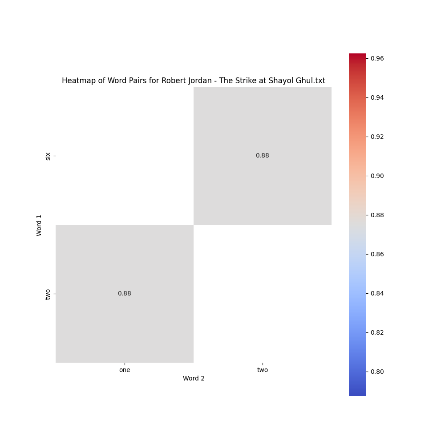
\includegraphics[width=\textwidth]{img/heatmap1.png}
        \caption{Distance 1}
        \label{fig:heatmap_1}
    \end{subfigure}
    \hfill
    \begin{subfigure}[b]{0.3\textwidth}
        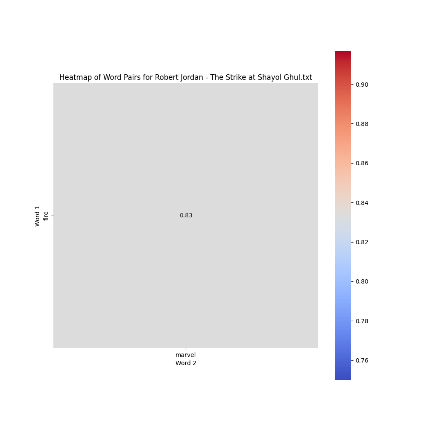
\includegraphics[width=\textwidth]{img/heatmap2.png}
        \caption{Distance 2}
        \label{fig:heatmap_2}
    \end{subfigure}
    \hfill
    \begin{subfigure}[b]{0.3\textwidth}
        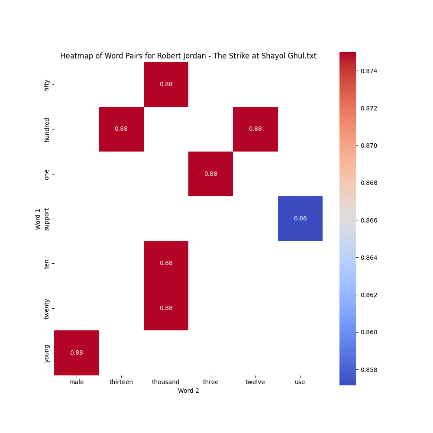
\includegraphics[width=\textwidth]{img/Heat Map3.png}
        \caption{Distance 3}
        \label{fig:heatmap_3}
    \end{subfigure}
    \caption{Heatmap of semantic similarity between word pairs at different distances.}
    \label{fig:heatmaps}
\end{figure}

\subsection{Scatter Plot}

We plot the semantic similarities of word pairs against their distance in the text. This can help visualize whether there is a relationship between semantic similarity and physical proximity of words.
According to the scatterplot graphs, the results of each book are similar to other books. It seems that there are fewer words with high semantic similarity at distances 1, 2, and 3. However, we did not obtain any particularly unique results from this graph.

\begin{figure}[H]
    \centering
    \begin{subfigure}[b]{0.3\textwidth}
        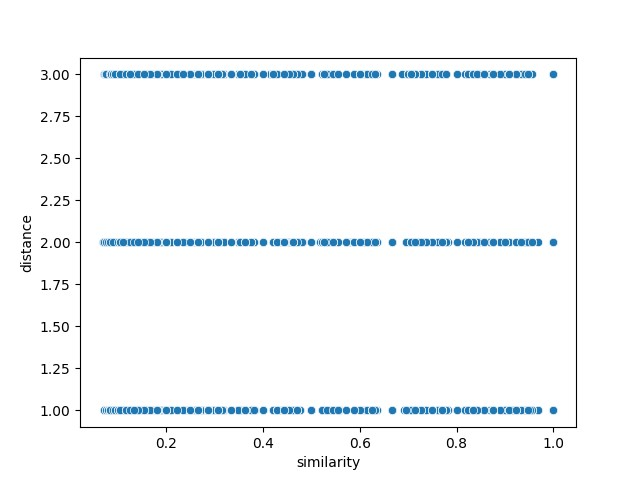
\includegraphics[width=\textwidth]{img/scatter_plot1.jpg}
        \caption{Distance 1}
        \label{fig:scatter_plot_1}
    \end{subfigure}
    \hfill
    \begin{subfigure}[b]{0.3\textwidth}
        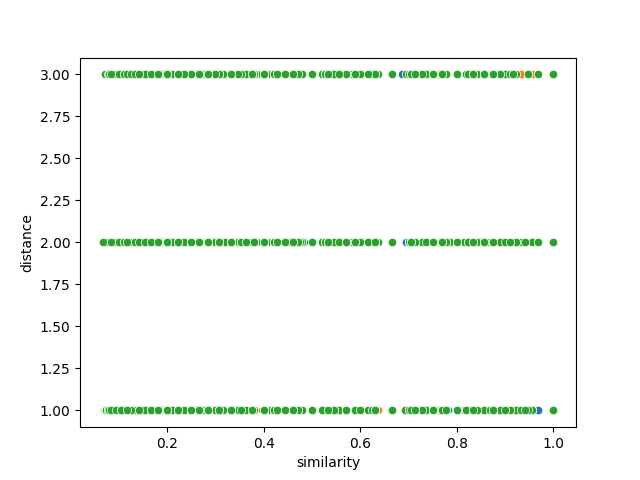
\includegraphics[width=\textwidth]{img/scatter_plot2.png}
        \caption{Distance 2}
        \label{fig:scatter_plot_2}
    \end{subfigure}
    \hfill
    \begin{subfigure}[b]{0.3\textwidth}
        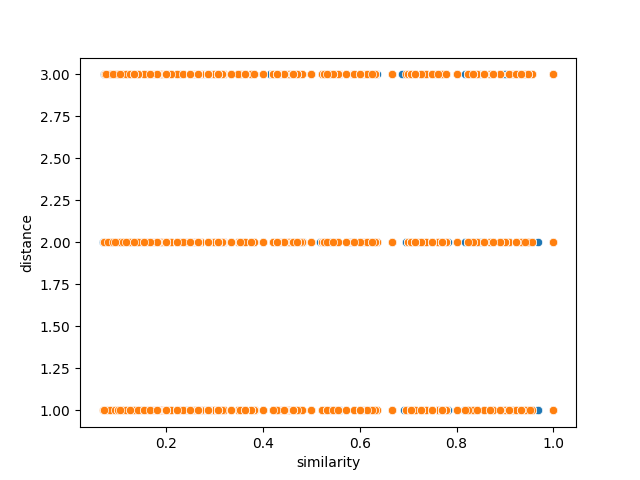
\includegraphics[width=\textwidth]{img/scatter_plot3.png}
        \caption{Distance 3}
        \label{fig:scatter_plot_3}
    \end{subfigure}
    \caption{Scatter plots of semantic similarity vs. distance between word pairs for different distances.}
    \label{fig:scatter_plots}
\end{figure}

\subsection{Word Cloud}

Create a word cloud where the size of each word corresponds to its average semantic similarity to other words in the document. It can provide an attractive visual representation of word importance based on similarity. Our understanding and analysis of these graphs can be that as the distance increases, the semantic similarity decreases and unrelated words appear more. However, Word Cloud helps us more than extracting important information about the degree of similarities in Different distances give more of an attractive visual representation of words.

\begin{figure}[H]
    \centering
    \begin{subfigure}[b]{0.3\textwidth}
        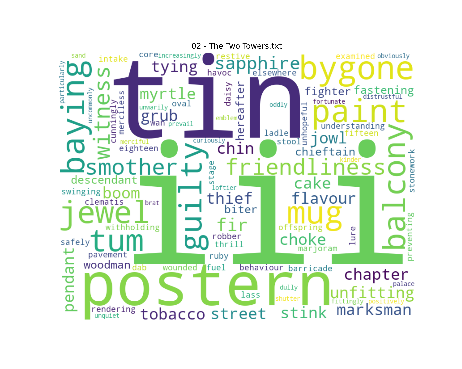
\includegraphics[width=\textwidth]{img/Word Cloud1.png}
        \caption{Distance 1}
        \label{fig:wordcloud_1}
    \end{subfigure}
    \hfill
    \begin{subfigure}[b]{0.3\textwidth}
        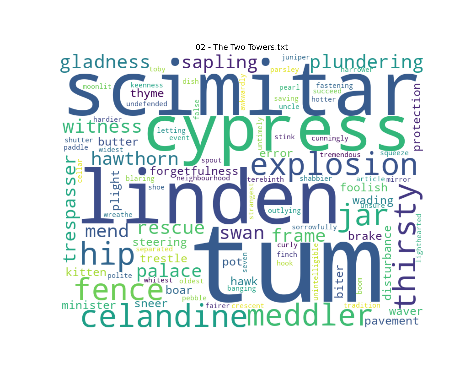
\includegraphics[width=\textwidth]{img/Word Cloud2.png}
        \caption{Distance 2}
        \label{fig:wordcloud_2}
    \end{subfigure}
    \hfill
    \begin{subfigure}[b]{0.3\textwidth}
        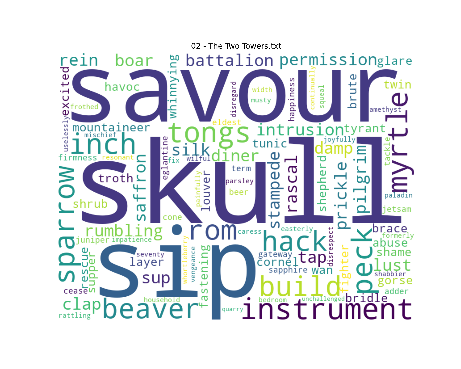
\includegraphics[width=\textwidth]{img/Word Cloud3.png}
        \caption{Distance 3}
        \label{fig:wordcloud_3}
    \end{subfigure}
    \caption{Word Clouds representing the average semantic similarity of words at different distances.}
    \label{fig:wordclouds}
\end{figure}

\subsection{Interactive Visualization}

We implemented an interactive visualization tool where users can explore the semantic similarities of word pairs by hovering over or clicking on specific elements in a graph.

\begin{figure}[H]
    \centering
    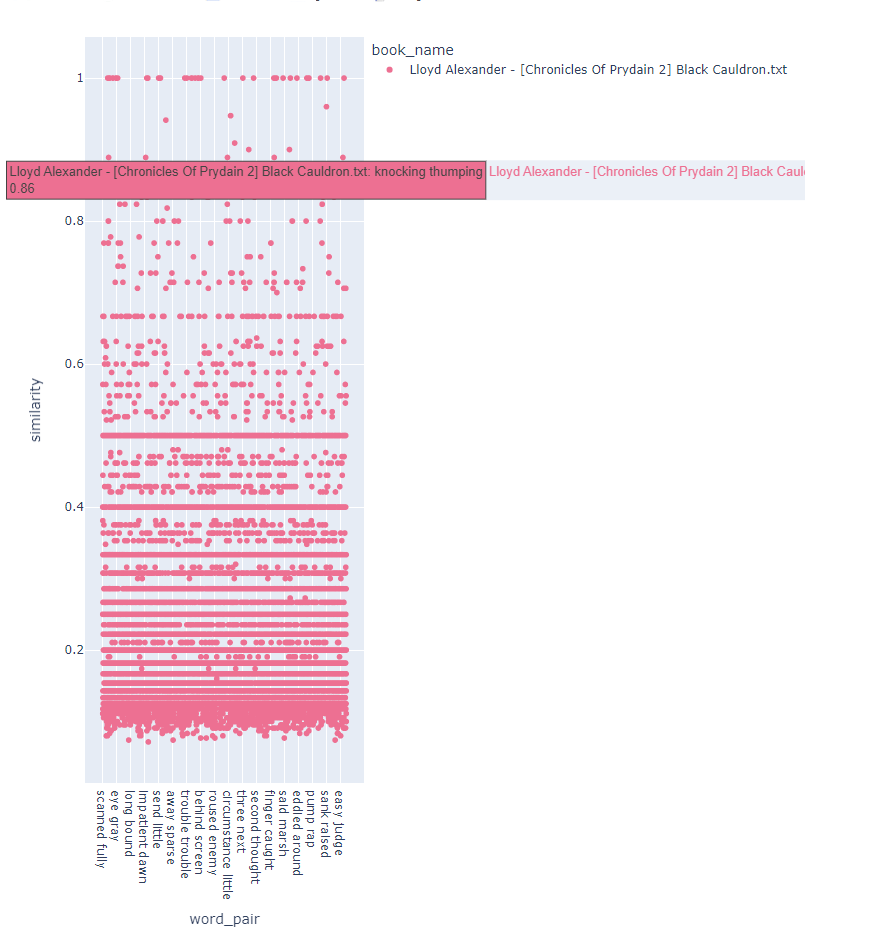
\includegraphics[width=1.0\textwidth]{img/Interactive Visualization.png}
    \caption{Interactive graph showing the degree of similarity of pairs of words.}
    \label{fig:interactive_visualization}
\end{figure}

\subsection{Bar Chart}

This bar chart shows the average semantic similarity of pairs of words at different distances, which helps to recognize the existence of patterns based on the distance between words. According to the size of 1, the second diagram is in the distance of 2, and the third diagram is in the distance of 3, and it is based on the degree of similarity between the pairs of words. From their analysis, we conclude that the smaller the distance between the pairs of words, the higher their semantic similarity. As the distance between words increases, they lose their semantic similarity, indicating that words close to each other have a stronger semantic connection.

\begin{figure}[H]
    \centering
    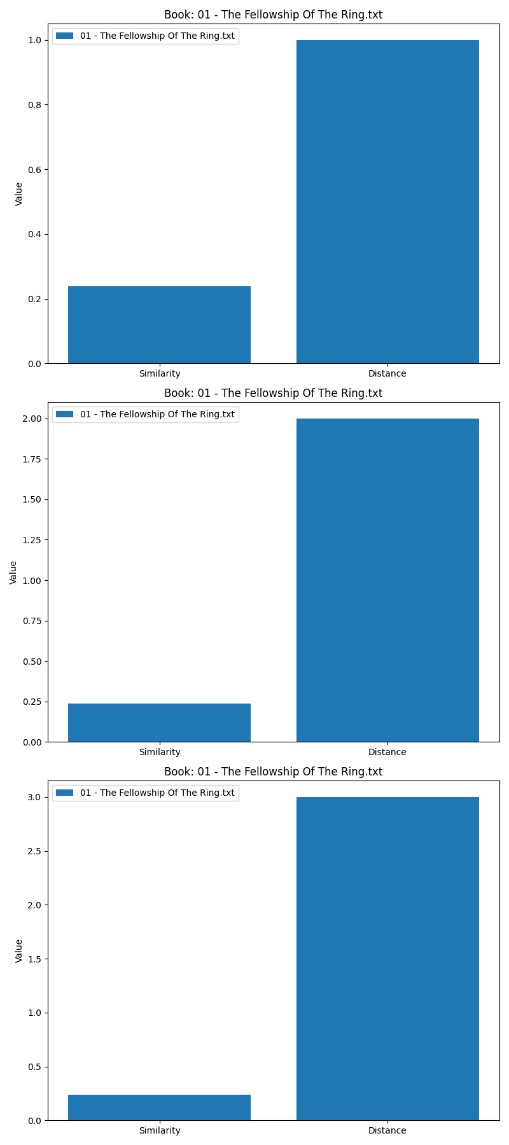
\includegraphics[width=0.5\textwidth]{img/bar_chart.jpg}
    \caption{Bar chart showing the average semantic similarity of word pairs at different distances.}
    \label{fig:bar_chart_1}
\end{figure}

\section{Conclusion}

In this paper, we calculated the semantic similarity of word pairs in the text of 86 famous English novels using the Wu-Palmer method in WordNet and analyzed them using different visualization methods. The results showed that the proximity of words to each other in the text has a direct relationship with their semantic similarity, which can be particularly useful in natural language processing tasks such as information retrieval, text classification, and machine translation. We used various techniques such as Heatmaps, Scatter Plots, Word Clouds, and Bar Charts to visualize the data, each providing different insights into the relationship between word proximity and semantic similarity. However, this method is time-consuming and complex to implement on a large scale, requiring further research to improve and optimize the process.

\end{document}
